\chapter{Design of Plutt}

\section{Goals of Plutt}

Plutt aims to improve on other micro front-end solutions regarding responsibilities and ownership in decision-making in an organization. The primary decisions plutt targets are: 1) deciding when to update a micro front-end; 2) deciding where and how to host a micro front-end. As a secondary goal, plutt aims to achieve this with no boilerplate code.

The primary reasoning originates from Michal Geer's organization model of highly decoupled vertically aligned teams, and the concept of independent deployability mentioned by Joel Denning, Luca Mezzalira, and Zackary Jackson. A development team that creates a micro front-end should be able to deploy an update whenever it best suits them. There also has to exist a mechanism for how to handle breaking changes, as breaking changes impact other teams. Teams that depend on a micro front-end should be able to decide when they want to update a micro front-end to a newer breaking version, as it can require refactoring in their source code. Without a mechanism for providing lock-step deployment, the decision of when to update is wrongfully always up to the team providing a micro front-end.

Luca Mezzalira's definition of micro front-ends include autonomy, which can extend into team autonomy in choosing technologies and hosting solutions. Most micro front-end solutions require that the dependent of a micro front-end has to know where and how to fetch a micro front-end. If a micro front-end changes its hosting solution, it requires synchronized updates between two teams, which contradicts autonomy. This contradiction can be solved by rerouting requests from the old location to the new location, but a more robust solution would be to provide access transparency to dependents. In a type-safe environment, access transparent solutions have to provide static type information about a micro front-end component.

To fulfill the mentioned goals, plutt provides the following properties:

\begin{enumerate}
    \item Lock-step deployment using semantic versioning
    \item Technology heterogeneity
    \item Access transparency
    \item Static type information\footnote{Don't forget to mention this}
\end{enumerate}

\section{Architecture}

% overall architecture (how many components are there, what are the main responsibilities of each component, etc)

Plutt is a build tool that generates client-side integrated micro front-end applications. Plutt uses a react component as input and outputs two artifacts: a \textit{Plutt Application} (composed of the original Component and a \textit{Wrapper}) and a \textit{Proxy}. To serve plutt applications plutt comes with a \textit{Plutt Server}. Figure \ref{fig:plutt-architecture} shows a comparison between a monolithic application and an application that uses plutt. A component can recursively include other components or JavaScript modules.

A plutt application is composed of a wrapper and a component. The wrapper makes the component mountable, unmountable, and exposes methods to propagate and update properties. A proxy knows how to fetch and use the corresponding plutt application. The proxy is included in a parent application and propagates property values and updates. To achieve technology heterogeneity, plutt generates a different framework native proxy for every supported framework. All necessary information about how to fetch and use a plutt application is inserted into the proxy at compile time. This makes the proxies access transparent. The proxys API is the same as the corresponding components API, and the parent application does not have to configure the location of the plutt application. Neither the team who provides the parent application or the team who provides the plutt application has to implement any code to fetch, mount, unmount, or propagate properties.

\begin{figure}
    \centering
    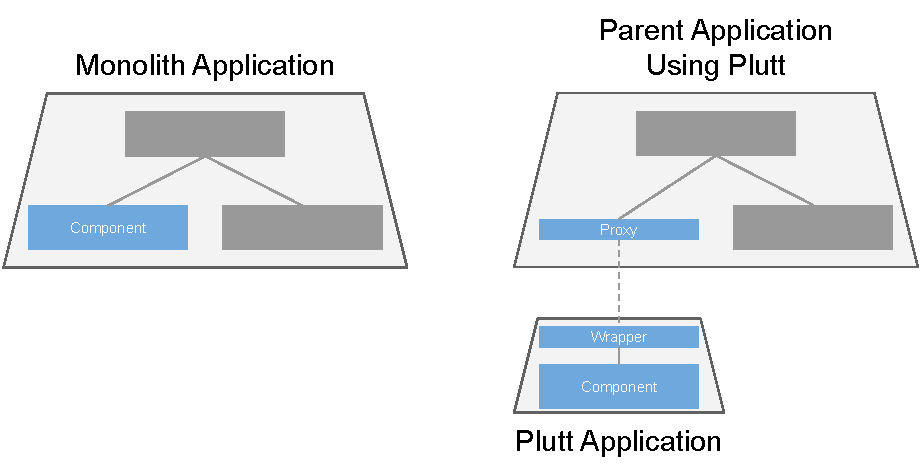
\includegraphics[width=\linewidth]{images/plutt-architecture.pdf}
    \caption{Plutt Architecture compared to an equivalent monolithic front-end application.}
    \label{fig:plutt-architecture}
\end{figure}

To facilitate lock-step deployment, plutt applications can be stored on a plutt server that automatically upgrades requests to the latest available plutt application that is non breaking. That way minor updates will automatically be published whenever a plutt application is updated, while breaking updates are implemented when a parent application is refactored. This gives every team the correct responsibilities that facilitates independent deployments.


\section{Details}
To understand how plutt works there are four perspectives that should be considered: Developing a plutt application, plutt application at run time, serving plutt applications, and using a plutt application.

\subsection{Developing a Plutt Application}

Developing a plutt application is not very different from developing a component in a monolithic application. Plutt provides build capabilites through a \ac{CLI}. When building, plutt starts with extracting the project name, version, and the public path that the application will be located at (host path). Plutt extracts this from a JSON document in the project directory (\texttt{package.json}).

Secondly plutt generates the application. It does this by generating the wrapper, which in turn imports the source component, and exports functions that mount the source component to a provided \ac{DOM} node, unmount the source component, and update the source component. Plutt then uses webpack to transpile and bundle the project into one JavaScript file. The name of the bundle is based on the project name and version, so that plutt server knows what asset and what version of the asset, the file contains.

If the source component is implemented using TypeScript, type information is extracted at this step, and type definition files are created. The proxies should be API equivalent to the source component so the same type definitions can be used for the proxies. Plutt only supports type definitions for the proxy of the same type as the source component, as type information is differently structured for different frameworks. This could be extended with sophisticated analysis and conversion.

Lastly the different proxies are generated. The proxies are generated with the host location of the plutt app hard coded. The location is a concatenation between the configured host path and the derived file name.

The proxy can be uploaded to a package registry that can be included in a parent application, and the plutt application has to be uploaded to a hosting location that is available by the end user, and the same location as previously configured.

\subsection{Plutt Application at Run Time}



\subsection{Serving Plutt Applications}

A plutt application can be uploaded to a static file server. If the same version and name is used every time, the plutt application could be updated by replacing the plutt application file on the file server. In this case the developers of the plutt application is the team that decides when the user facing web page is updated, which could introduce problems if an update introduces breaking changes.

Another option is to keep all versions of a plutt application on a static file server, and use the unique file names they are generated with. This is done by updating the configured version every time a new version of a plutt app is created. As every version of the proxies only points to a unique plutt application, new versions of the plutt application will only be user facing when the developers of the parent application decides to update their proxy.

An optimal solution would be that the team providing a micro front-end decides when non breaking updates are published into production, and the parent application team decides when to update to newer breaking versions. In other words the best solution would be to provide both independent deployments, and API safety using lock-step deployment. Plutt server is a plutt application repository that provides version safe independent deployments.

Whenever plutt server receives a request, the server examines if there is a higher version of the requested asset that is non breaking. If there exists a more recent non breaking version, plutt server will upgrade the request to the highest available non breaking version. This means that the users of a plutt application will always get at least the version that existed when they included the proxy in there application, but could be provided with updates as long as they are non breaking. The providers of a plutt application own the responsibility of publishing non breaking updates. Whenever a breaking update is introduced, the teams can use lock-step deployment to gradually introduce the new update. For the team that uses a plutt application, this means updating their imported proxy.

\subsection{Using a Plutt Application}


\section{Implementation}

answer to RQ1


\chapter{Old Design of Plutt}

\textbf{Write something short here}

\section{Goals of Plutt}

Plutt aims to improve on other micro front-end solutions regarding responsibilities and ownership in decision-making in an organization. The primary decisions plutt targets are: 1) deciding when to update a micro front-end; 2) deciding where and how to host a micro front-end. As a secondary goal, plutt aims to achieve this with no boilerplate code.

The primary reasoning originates from Michal Geer's organization model of highly decoupled vertically aligned teams, and the concept of independent deployability mentioned by Joel Denning, Luca Mezzalira, and Zackary Jackson. A development team that creates a micro front-end should be able to deploy an update whenever it best suits them. There also has to exist a mechanism for how to handle breaking changes, as breaking changes impact other teams. Teams that depend on a micro front-end should be able to decide when they want to update a micro front-end to a newer breaking version, as it can require refactoring in their source code. Without a mechanism for providing lock-step deployment, the decision of when to update is wrongfully always up to the team providing a micro front-end.

Luca Mezzalira's definition of micro front-ends include autonomy, which can extend into team autonomy in choosing technologies and hosting solutions. Most micro front-end solutions require that the dependent of a micro front-end has to know where and how to fetch a micro front-end. If a micro front-end changes its hosting solution, it requires synchronized updates between two teams, which contradicts autonomy. This contradiction can be solved by rerouting requests from the old location to the new location, but a more robust solution would be to provide access transparency to dependents. In a type-safe environment, access transparent solutions have to provide static type information about a micro front-end component.

To summarize, plutt could fulfill its goals by providing the following qualities:

\begin{enumerate}
    \item Lock-step deployment using semantic versioning
    \item Technology heterogeneity
    \item Access transparency
    \item Static type information\footnote{Don't forget to mention this}
\end{enumerate}

\section{Architecture}

Plutt is a build tool that generates client-side integrated micro front-end applications. The input is a react component and plutt outputs two artifacts\footnote{Is artifact the right word?}: a \textit{Plutt Application}, containing a \textit{Wrapper}, and a \textit{Proxy}. To serve plutt applications plutt comes with a \textit{Plutt Server}. Figure \ref{fig:plutt-architecture} shows a comparison between a monolithic application and an application that uses plutt. A component can recursively include other components or JavaScript modules.


\begin{figure}
    \centering
    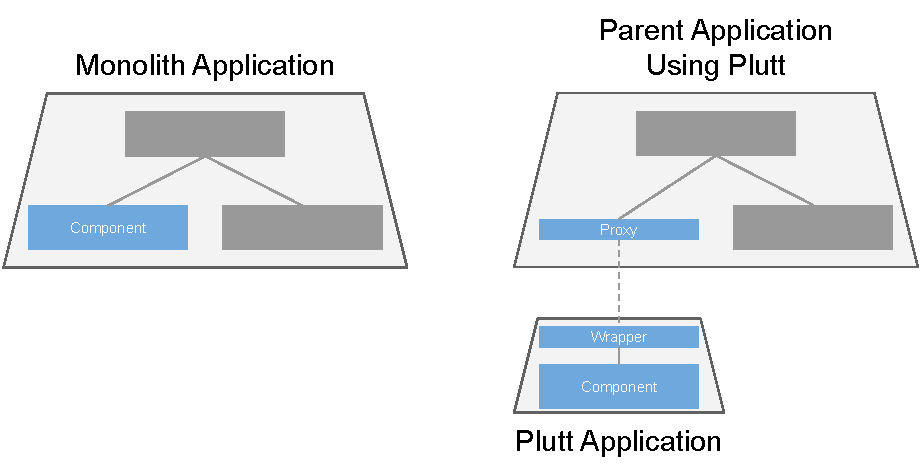
\includegraphics[width=\linewidth]{images/plutt-architecture.pdf}
    \caption{Plutt Architecture compared to an equivalent monolithic front-end application.}
    \label{fig:plutt-architecture}
\end{figure}

\subsection{Plutt Application}
The input component is wrapped in a wrapper that plutt generates. The wrapper is a JavaScript module that exposes functions to mount and unmount the component on an HTML element. The wrapper also propagates properties to the component and exposes a function to update the properties. The wrapper and component is compiled into one bundle by plutt, which is the plutt application. Plutt only supports components to be react components, but can be extended to support components implemented using other frameworks.

This bundle can be fetched in run-time using dynamic imports in JavaScript, like Joel Denning mentioned\footnote{Mention dynamic imports and esmodules}, and mounted on an HTML element. If a parent application fetches a plutt application at run time, the plutt application can be replaced in run time, which enables independent deployments.


\subsection{Proxy}
When compiling a plutt application, plutt compiles proxies that knows how to fetch, mount and unmount a plutt application. The proxies can also receive properties and property updates which it propagates to the mounted plutt application. To accomplish this plutt has to know where the plutt application will be hosted at compilation-time, which is inserted into the proxies.

The proxies are generated to be included in the parent application, which is why there are multiple different proxies. There is one proxy for every supported framework, which at this point is React and Vue. The proxy is a framework-native component which can be used exactly as if it was the original component. Code-wise it looks exactly the same as if the parent application would include the original component, given that the component is implemented using the same framework. The proxy provides access transparency and technology heterogeneity.

As the proxy does not contain business logic it works with any non-breaking version of the corresponding plutt application. Independent deployments can be achieved by replacing only the plutt application on the hosted location. The proxy does not have to be updated in the parent application at the same time.

\subsection{Plutt Server}
The plutt application could be hosted on a static file server, but that does not provide lock-step deployment. Every time a plutt application is replaced, the corresponding proxy would fetch the latest version, even if the latest version contains a breaking update. This gives the full ownership of updating to the team who is responsible for the plutt app, which could lead to the team developing the parent application to be forced to update their application at a time that does not suit them.

To solve this plutt appends the version to the filename of the plutt application, every time plutt compiles a plutt application. Every version of the plutt application should result in a unique file name, provided semantic versioning is used. Instead of replacing the plutt application at the host location, every new file can be appended to a repository with a unique hosting location. The parent application will get the version that was compiled with the proxy that is included. Table \ref{table:plutt-configuration} shows an example configuration and Table \ref{table:plutt-configuration-result} shows what values would be derived.

\begin{table}
\centering
\caption{Configuration values inputed into plutt}
\label{table:plutt-configuration}
\begin{tabular}{|l|l|}
\hline
name      & banner                           \\ \hline
version   & 2.1.1                            \\ \hline
host path & https://banners.com/plutt/banner \\ \hline
\end{tabular}
\end{table}

\begin{table}
\centering
\caption{The resulting values derived from the configuration values in Table \ref{table:plutt-configuration}. File name is the file name of the plutt application bundle, and full host path is the path that the proxy will fetch from.}
\label{table:plutt-configuration-result}
\begin{tabular}{|l|l|}
\hline
file name      & banner.v2.1.1.js                                  \\ \hline
full host path & https://banners.com/plutt/banner/banner.v2.1.1.js \\ \hline
\end{tabular}
\end{table}

The full ownership of updating the plutt application is moved to the team that develops the parent application. Using this method, the parent application team will not get non breaking updates automatically, which is also suboptimal. The optimal solution would be that the team providing a micro front-end decides when non breaking updates are published into production, and the parent application team decides when to update to newer breaking versions. To solve this issue, plutt comes with a server for serving plutt applications in a semantically safe manner.

Whenever plutt server receives a request, the server examines if there is a higher version of the requested asset that is non breaking. If there exists a more recent non breaking version, plutt server will upgrade the request to the highest available non breaking version.

This means that the users of a plutt application will always get at least the version that existed when they included the proxy in there application, but could be provided with updates as long as they are non breaking. The providers of a plutt application own the responsibility of publishing non breaking updates. Whenever a breaking update is introduced, the teams can use lock-step deployment to gradually introduce the new update. For the team that uses a plutt application, this means updating their imported proxy.

\subsection{Type safety}



\subsection{Summary or something}

\textbf{Write a short summary here}

For sake of open-science, the code is made publicly available at \textbf{insert link here}